%\documentclass[preprint,tightenlines,showpacs,showkeys,floatfix,
%nofootinbib,superscriptaddress,fleqn]{revtex4} 
\documentclass[tightenlines,floatfix,nofootinbib,superscriptaddress,fleqn]{revtex4} 
%\documentclass[aps,epsfig,tightlines,fleqn]{revtex4}
\usepackage{kotex}
\usepackage[HWP]{dhucs-interword}
\usepackage[dvips]{color}
\usepackage{graphicx}
\usepackage{bm}
%\usepackage{fancyhdr}
%\usepackage{dcolumn}
\usepackage{defcolor}
\usepackage{amsmath}
\usepackage{amsfonts}
\usepackage{amssymb}
\usepackage{amscd}
\usepackage{amsthm}
\usepackage[utf8]{inputenc}
%\pagestyle{fancy}

\begin{document}

\title{\Large 2022년 2학기 물리학 II}
\author{김현철\footnote{Office: 5S-436D (면담시간 매주
    수요일-16:15$\sim$19:00)}} 
\email{hchkim@inha.ac.kr}
\affiliation{Hadron Theory Group, Department of Physics,
  Inha  University, Incheon 22212, Republic of Korea }
\date{Autumn Semester, 2022}

\maketitle

{\color{red} {\bf Due date:} 2022년 11월 2일  15:00-16:15 }
\vspace{1.cm}

\noindent \textbf{ 주의: \color{blue} 단 한 번의 부정행위도 절대
  용납하지 않습니다. 적발 시, 학점은 F를 받게 됨은 물론이고,
  징계위원회에 회부합니다. One strike out임을 명심하세요.} 
\\
\\

{\bf 학번:} \hspace{4cm}
{\bf 이름:} 

\section*{\large Quiz 14}
\noindent {\bf 문제 1 [20pt]}
빛이 물의 표면에 $53.0^\circ$로 입사하였다. 물의 굴절률이 1.33일 때, 물
내부로 굴절된 빛의 굴절각은 얼마인가? 또 입사각과 굴절각의 합은
얼마인가? 이 경우 물의 표면에서 반사된 빛은 한 방향으로 편광되어
있음을 증명하여라. 
\newpage

\noindent {\bf 문제 2 [20pt]}
곡률반지름이 20.0 cm인 볼록거울의 축상에서 14.0 cm 앞부분에 점광원이
놓여 있다면 상이 생기는 지점은 어디인가? 이 상은 실상인가 아니면 허상인가?
\newpage

\noindent {\bf 문제 3 [50pt]}
그림~\ref{fig:1}에서 직각 모서리 프리즘 (corner cube prism) 2개의 거울을
직각으로 붙여 만든 그릇에 물을 담은 형태를 생각하자. 빛이 수면에
수직으로 입사하는 경우, 빛은 물을 지나 1개의 거울면에서 반사하고 다시
다른 거울면에서 반사하여 물을 빠져나올 것이다.
\begin{figure}[htp]
  \centering
  \includegraphics[scale=0.5]{qfig14-1.png}
  \caption{\textbf{문제 3}}
  \label{fig:1}
\end{figure}
\begin{itemize}
\item[(가)] 이때 두 번 반사된 빛은 원래의 입사광과 평행하게 되돌아가게
  된다는 것을 증명하여라.
\item[(나)] 빛이 비스듬하게 입사하는 경우에도 반사된 빛은 항상 입사한
  빛에 평행이 된다는 것을 증명하여라.
\item[(다)] 정육면체 유리 덩어리의 모서리를 45° 각도로 잘라내어
  만들어진 피라미드 형태의 유리에 대 해서도 위의 관계가 성립되는 것을
  보여라. 이 때 유리의 굴절률이 1.45라고 가정하고 전반사 조건을
  고려하여라. 실제로, 사고 예방을 위해서 자전거 등에는 밤에 다른
  자동차의 불빛에 의해 빛나게 되는 물체를 부착하는데, 이 물체는 이 와
  같은 작은 피라미드 모양의 플라스틱을 여러 개 붙여 놓은
  형태이다. 자동차 양끝의 방향지 시등 커버도 이와 같이 되어 있다.  
\end{itemize}
\newpage

\noindent {\bf 문제 4 [100pt] {\color{red} (난이도 상)}} 
그림~\ref{fig:2}에서는 수영장 수면 위 $d_1=250$ cm 위에 매달려 있는
작은 전구를 보여준다. 수영장의 깊이는 $d_2=200$ cm이다. 수영장
바각에는 큰 거울이 놓여 있다. 이 전구의 상은 수면에서부터 밑으로 얼마나 멀리
놓여 있는가? 
\begin{figure}[htp]
  \centering
  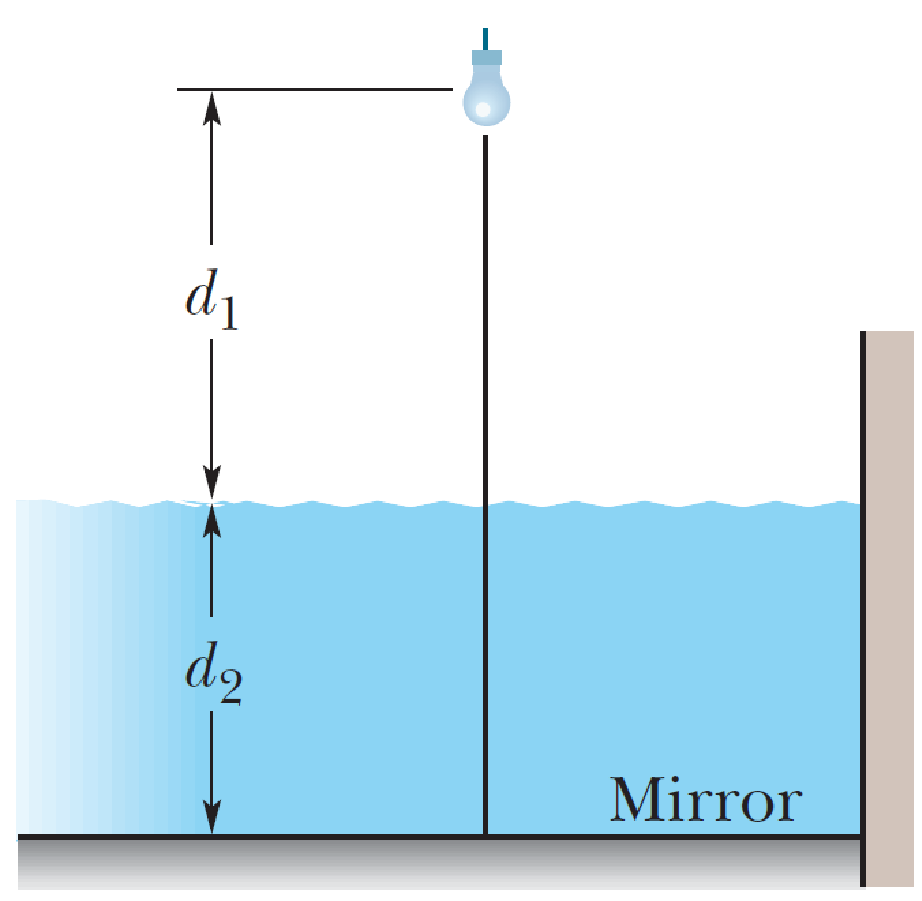
\includegraphics[scale=0.35]{qfig13-4-20221031.pdf} 
  \caption{\textbf{문제 4}}
  \label{fig:2}
\end{figure}

\begin{itemize}
\item \noindent 귀띔 1: 빛살(ray))는 전구를 지나는 수직축에 가까이 있다고
가정하여라. 그러면 $\sin\theta\approx \tan\theta \approx \theta$와
같은 근사를 쓸 수 있다.
\item \noindent 귀띔 2: 다음 그림~\ref{fig:3}을 참조해서 문제를 푸세요.
\end{itemize}
\begin{figure}[htp]
  \centering
  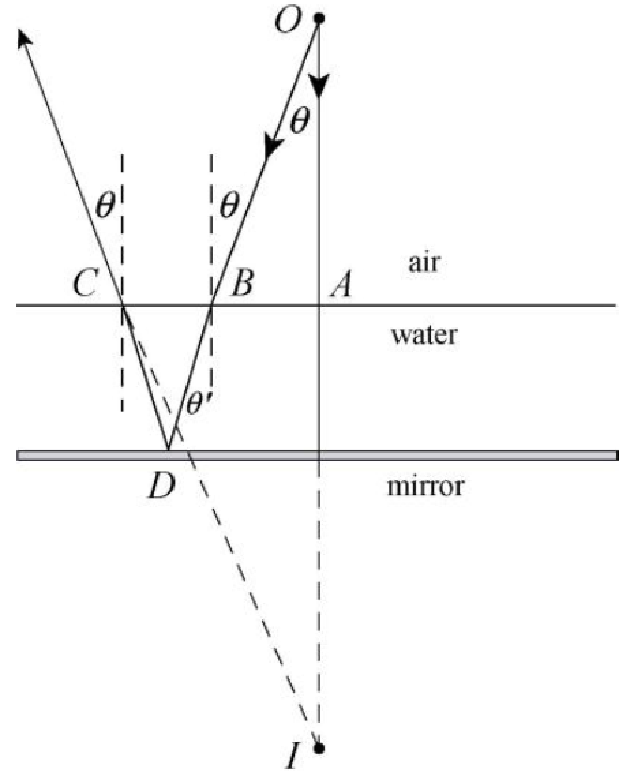
\includegraphics[scale=0.5]{qfig13-4-1-20221031.pdf} 
  \caption{\textbf{문제 4 귀띔}}
  \label{fig:3}
\end{figure}

\vspace{0.3cm}

\noindent \textbf{\color{blue} 이 문제를 푼 학생에게는 10,000원에
  해당하는 커피 쿠폰을 제공합니다.}  
\newpage
{\color{gray} [문제 풀이 쪽]}
\end{document}

